\documentclass[../report.tex]{subfiles}

\begin{document}
\section{Problem Description}
University of Nottingham Malaysia has a mobile application called \textit{UNM Instatt} to aid lecturers and students take attendance during academic sessions. Instead of signing on paper, students will press an icon within a limited time frame to indicate themselves as present after the lecturer has turned on the signing-in feature. Students will get to monitor their attendance rate and check their timetable schedule in the application and likewise for lecturers. 

However, some students might forget to sign-in even though they attended the class. In that case, lecturers need to sign in manually for them. There is also no notification when attendance is opened to be signed and students might miss the signing time frame. The process of attendance taking is also disruptive to the academic process as students need to open the application every time to record attendance.

\section{Proposed Solutions}
This project aims to create an application called Beam that can automatically record attendance of students in class. This application will run in the background and use Bluetooth Low Energy (BLE) to detect the students’ proximity to lecturer or students who already recorded attendance. Once the lecturer enabled sign-in of attendance on his device, that device will send a token through BLE to other BLE-enabled devices nearby. The application will communicate with a server once the token has been received and the server will record attendance for the students. Once the student’s attendance is recorded, the student’s device will act as a beacon which shares the lecturer’s token to nearby devices so that students whose devices are out of the lecture’s device Bluetooth range could receive the lecturer’s token.  There will be a separate website which handles the timetable scheduling and registration of lecturer and student details.  

Furthermore, the application will notify students to turn on Bluetooth once attendance is open to sign in. When the device received a token from the lecturer or from other present students, the application will record timestamps to ensure attendance record matches the actual timetable.

\begin{figure}[H]
\centering
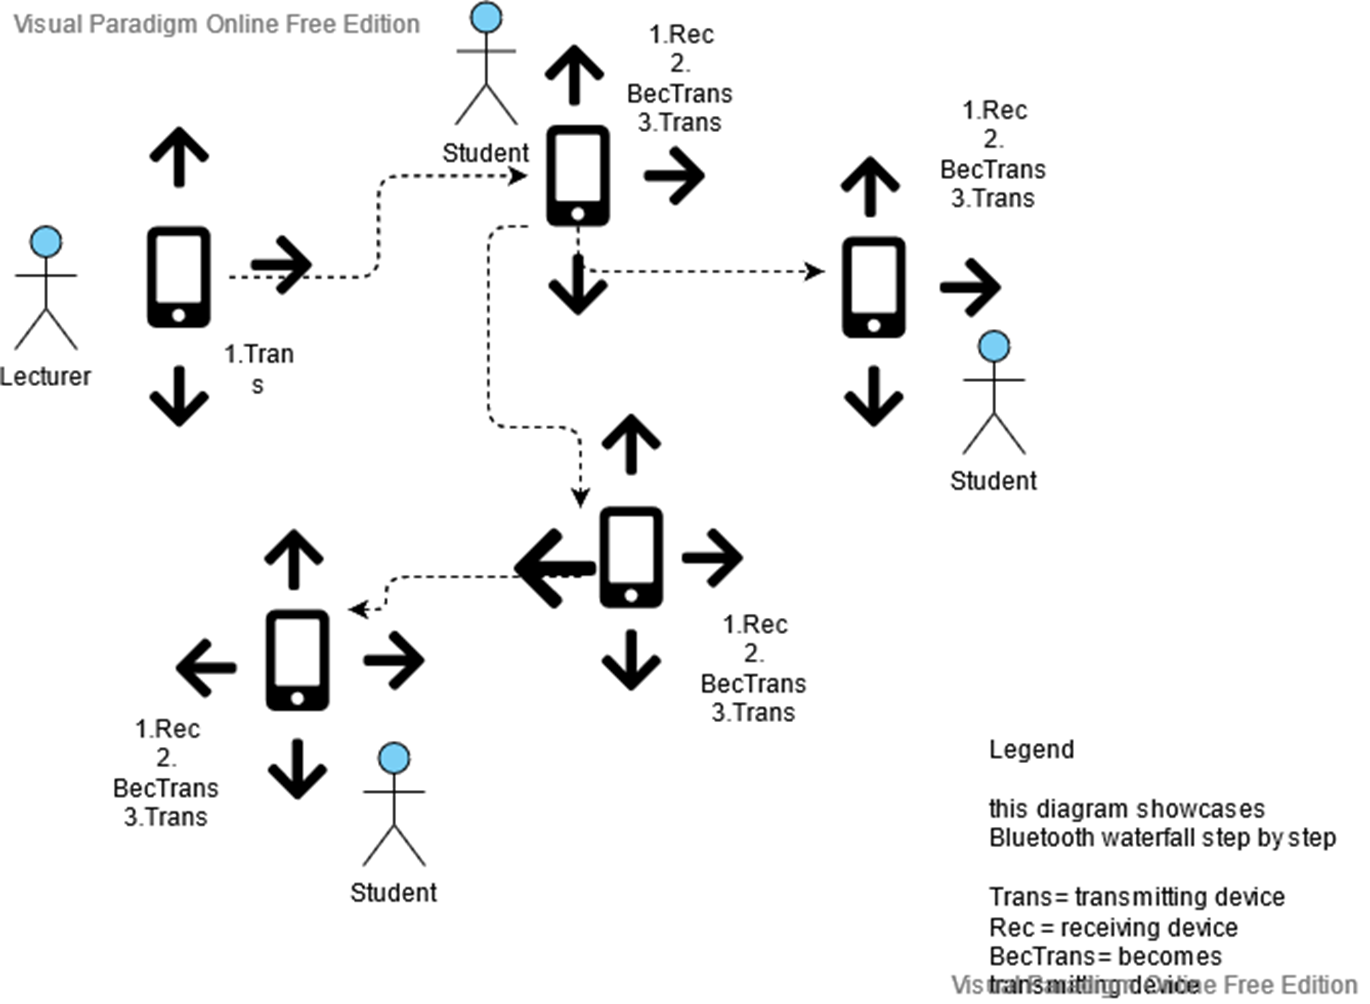
\includegraphics[width=.75\textwidth]{./images/02/02-solution-design.png}
\caption{Trans=Transmitting device, Rec=Receiving device, BecTrans=Becomes Trans}
\label{fig:solution-design}
\end{figure}

\section{Qualifications and Limitations}
One of the limitations of this application is that it could not detect proxy devices. Students who will not attend class can just hand their devices over to their friends who will attend to sign their attendance. Unless the lecturer counts the number of physical students in the class and tally with the number of students in the attendance record, which is a time-consuming process, students can take attendance with the application on behalf of their friends. If there is a separate device, such as an infrared sensor, that can detect the number of physical students in class automatically, then proxies can be eliminated, albeit at a high monetary cost. Furthermore, students who have already taken attendance can bring their devices to their friends outside the classroom to record attendance for them. Some students may turn off Bluetooth after taking attendance to save on battery consumption. Without Bluetooth, the device cannot act as a beacon for other students’ who have not taken attendance.

\section{Development Constraints}
Since this project is not commissioned by University of Nottingham Malaysia (UNM), the application will be linked with an artificial database instead of the real UNM student registry. Even though the data used in this project does not identify with any real user, the data processed will be encrypted as a good practice of data handling.

Testing cannot be performed in the university making it significantly harder to test for security requirements such as leakage of personal data to unauthorised parties amongst others. 

The use of an artificial database and the fact that the app will not be used by multiple students means that the app will never be tested on many devices making it considerably harder to test for several performance requirements, for instance how smooth the app runs on different Android devices or different networks.

\section{Target Audience}
This project aims to improve the existing attendance management application of \textit{UNM Instatt}. Hence, this application is created for UNM lectures and students.
\end{document}